A wide variety of reactions may produce {\IP}s at colliders, and, if the mediators of the interaction are light enough to be produced on-shell, collider experiments are particularly suited to discovering and characterizing the interactions responsible.  Meanwhile, connecting a collider experiment's discovery or non-discovery of {\IP}s to dark matter requires direct and indirect detection experiments, where galactic dark matter collides with a terrestrial target, or extragalactic dark matter annihilates.

Making this connection requires that one assumes a particle physics model.
Within a given model and under well-specified assumptions, the information obtained in a collider experiment can be related to the information obtained in direct, indirect, and astrophysical probes, and vice versa.
One can then compare and contrast the different types of information, e.g., to understand where a DM discovery in current DD searches could be further explored with mediator studies at the LHC, and where, amongst the multitude of possible signals, collider searches might focus effort.

In the following, we outline a strategy adopted by the ATLAS and CMS experiments when making comparisons with astrophysical observations (e.g., where is a model consistent with the present DM density in the universe), DD, and ID results. We discuss the assumptions made in the relic density calculation and in relating reactions for {\IP}s to reactions of DM.

\subsection{Comparing LHC constraints from visible and invisible searches with non-collider results}

The ATLAS and CMS collider results typically appear as constraints on production cross sections of specific processes, which are then interpreted as statements about the fundamental parameters of a simplified model (masses, couplings), Within the model, information on the parameters can then be extrapolated to statements about the non-collider observable of interest---for example, the WIMP-nucleon scattering cross section for DD, or the thermal relic density.
In Ref.~\cite{Boveia:2016mrp}, the LHC Dark Matter Working Group provides an in-depth discussion of how to perform these extrapolations.
Recently, most general LHC search results have selected a single, specific set of BSM-mediated simplified models for extrapolation, due to their immediate relevance with the first 13~TeV collision data. But many other models can be used~\footnote{For reinterpretation of LHC results and their comparisons to DD and ID for scalar and pseudoscalar mediators, also in the context of 2HDM, see e.g.~\cite{Athron:2017kgt,Banerjee:2017wxi,Bell:2016ekl}}, and published searches typically provide some form of model-agnostic results for this purpose.


As an example, CMS has extrapolated the parameter exclusions obtained by a recent set of searches to the spin-independent WIMP-nucleon cross section of a direct detection experiment.
The result, Fig.~\ref{fig:SICMS}, with a selection of DD results also shown for comparison, illustrates some general features of many such comparisons.
For spin-independent scattering, LHC searches for heavy {\IP}s are generally in the position of confirming non-observation of DM in DD searches, whereas LHC invisible particle searches are sensitive to arbitrarily light {\IP}s while DD searches are not, and at intermediate DM masses both LHC and DD experiments have great potential for a discovery and could verify each other's claims.
For spin-dependent DD scattering (e.g., an axial-vector-mediated model), because the LHC signals are relatively insensitive to the Lorentz structure of the interaction while the DD signals are suppressed, similar plots show that LHC searches play a more powerful role relative to the DD searches over a wide range of invisible particle masses. 

In the same way, one can compare collider and ID results using simplified model benchmarks. In traditional comparisons, only one DM annihilation state at a time has been used for the comparison of collider and ID results (e.g. $b\bar{b}$, see for example~\cite{Agrawal:2014una}) but one can also compare ID and LHC results for models annihilating to multiple final state fermions.~\cite{Carpenter:2016thc}.

Recently, some DD and ID collaborations have adopted the benchmark simplified models being used by ATLAS and CMS, see e.g.\cite{PhysRevLett.118.251301,Balazs:2017hxh}.
IceCube and other experiments have used constraints from a MSSM scan, see e.g.~\cite{Aartsen:2016zhm}. The pMSSM is also a good framework to highlight the complementarity of LHC, direct and indirect detection experiments, as shown in e.g. Ref,~\cite{Cahill-Rowley:2014twa} and discussed later. %CD: m

\begin{marginnote}[]
\entry{The LHC Dark Matter Working Group}{provides  for the translation of LHC limits to DD and ID in~\cite{Boveia:2016mrp}, as well as reference sets of simplified models, calculations of relic density, and other tools to standardize such comparisons~\cite{githubDMWG}.} 
\end{marginnote}. 

It must be underlined that the exclusion regions obtained in this way will depend strongly on the assumption of the model.
The extrapolations are done with full knowledge that the simplified model is merely a crude guess, and one must be careful not to over-generalize.
More so, neither this procedure nor the simplified models themselves account for effects outside the model, such as interference and mixing with SM boson and quarkonia resonances, or the evolution of the operators in the model from the LHC collision energies to other energy scales~\cite{DEramo:2014nmf}.
Moreover, all experimental results, be it from DD, ID or collider, are affected by experimental and theoretical uncertainties that are not displayed here.


\begin{figure}[!htpb]
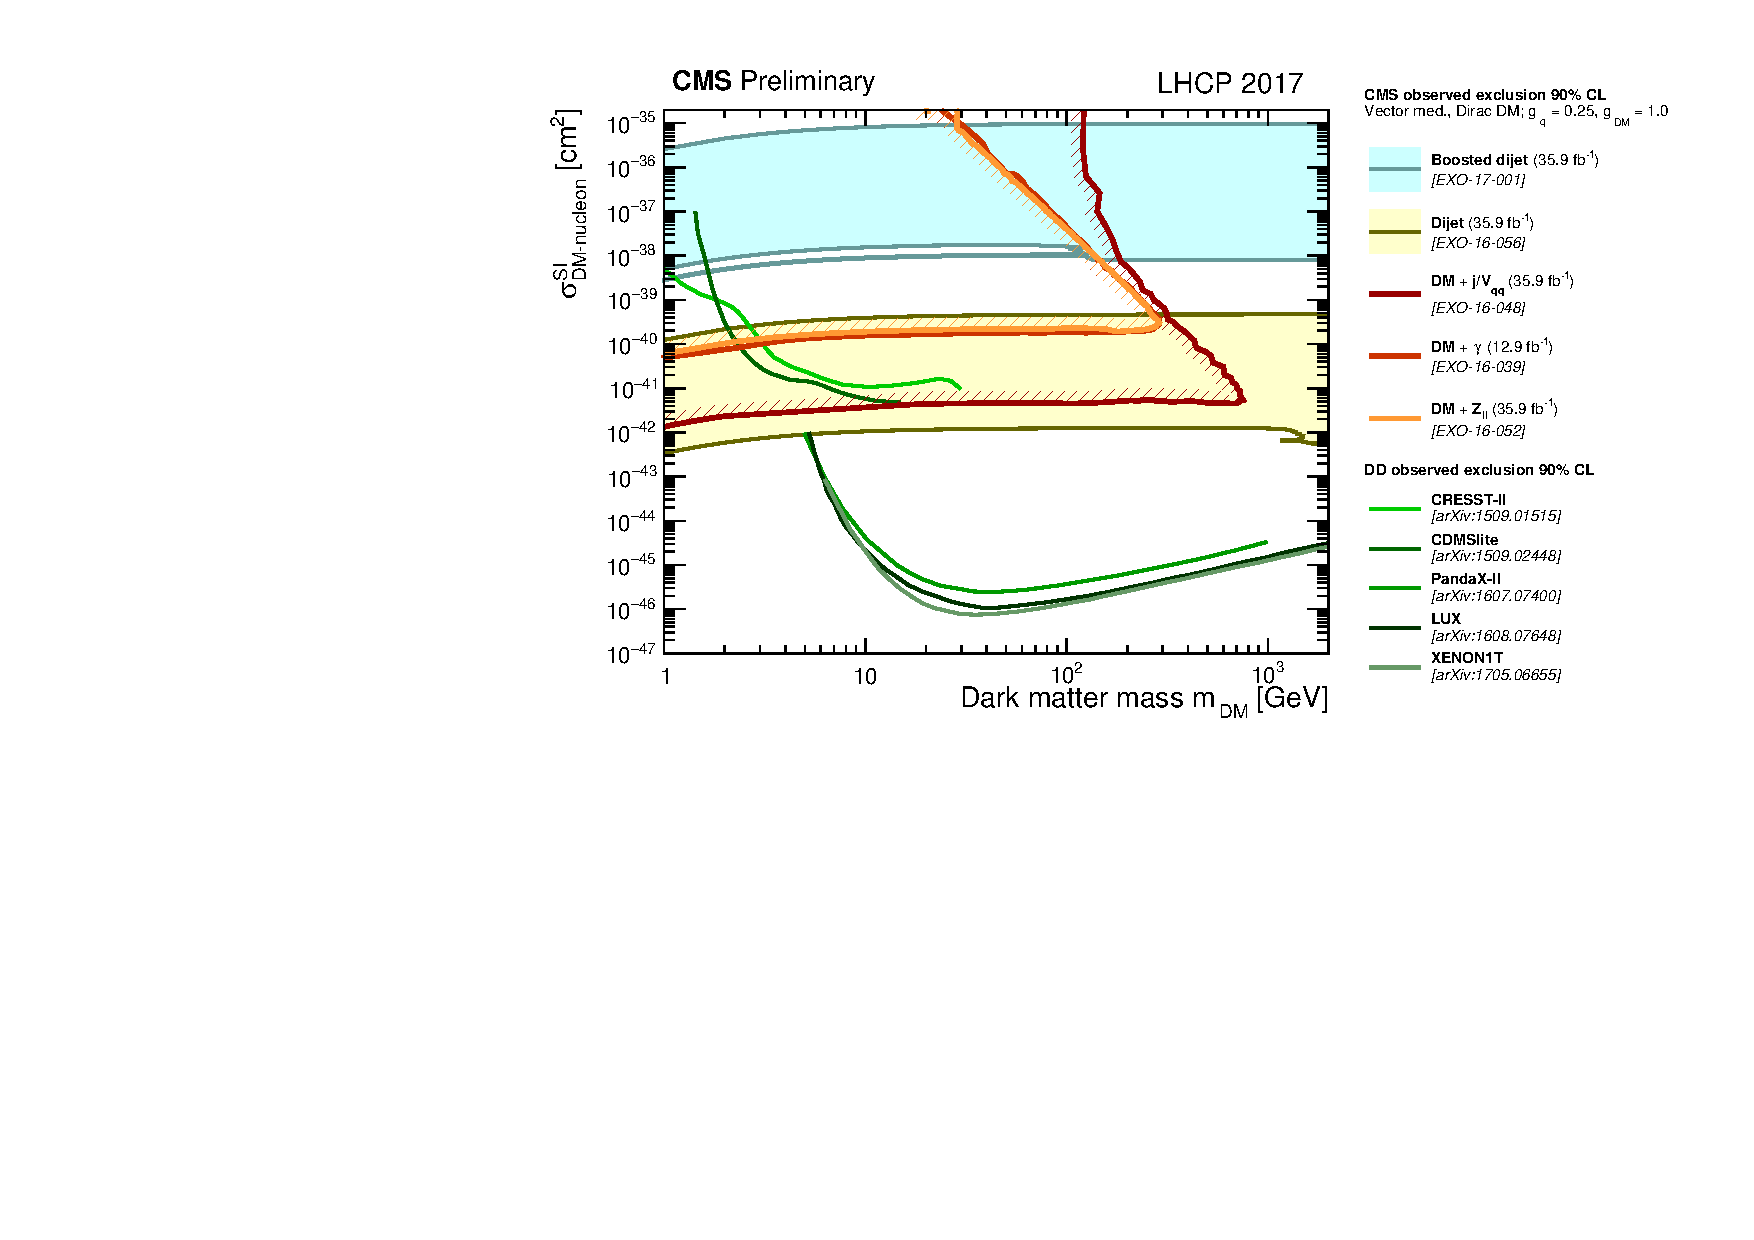
\includegraphics[width=0.9\textwidth]{figures/SI_CMSDD_Summary}
\caption{The 90\% CL constraints from the CMS experiment in the \mdm-spin-independent DM-nucleon plane, for a vector mediator, Dirac DM and couplings \gq = 0.25 and \gdm = 1.0, compared with DD experiments. From~\cite{CMSSummary}.}
\label{fig:SICMS}
\end{figure}

\subsection{Relic density considerations}
Absent a signal in non-collider experiments, the ability of a model to link its {\IP}s with the observed DM abundance is key to distinguishing it from other types of models of physics beyond the Standard Model.
Making this link, however, requires extrapolating from the present day to the early universe along an increasingly tenuous chain of assumptions.
For simplified models, this is especially problematic, because the model is designed to describe collider-scale processes; it may not even contain the interactions relevant in the early universe.
Nevertheless, it is interesting to examine where a model can make the link, even if in limited situations~\cite{Busoni:2014gta,Catena:2017xqq}.
For example, for the general simplified models in Sec.~[fix], one can compute with programs such as MadDM and MicrOMEGas~\cite{Backovic:2015cra,Barducci:2016pcb} the DM abundance for a standard thermal relic assuming that the interaction described by the simplified model is the one responsible for setting the relic density.
Often, e.g. Fig.~\ref{fig:sensitivityComparison}, ATLAS and CMS supplement their results with contours indicating where within a model this procedure obtains the correct dark matter density of $\omega_c = 0.12 h^2$.
Where the model cannot reproduce the correct abundance, it is an indication that either the model requires additional ingredients beyond those included in the simplified model, or that the chain of assumptions is incorrect~\cite{Bernal:2017kxu}.
